\documentclass[a4paper,10pt]{article}
\usepackage{listings}
\usepackage{graphicx}
\usepackage{bold-extra}
\usepackage{mathtools}
\usepackage{amssymb}
\usepackage{setspace}

\newcommand{\br}{\\[10pt]}
\let\emptyset\varnothing
\setstretch{1.3}

\lstset{ %
  frame=single,
  numbers=left,
  language=Ruby
}

\begin{document}
  \title{Computing Shapley Values in the English Premier League}
  \author{Paul Fletcher-Hill}
  \maketitle
  \section*{Introduction}
  In 1953, Lloyd Shapley introduced the concept of a Shapley value for coalitional games. Using four convenient axioms, the innovation allows the calculation of a unique distribution of the game’s surplus among its players, representative of their marginal power. The Shapley value has successfully been used in many political and economic games. In soccer, like many other sports, rating players is often a shallow and arbitrary process. Simple metrics, such as goals, shots or saves, are easily digestible, but they hardly encapsulate the actual value of a player while he is on the field. This paper attempts to apply the Shapley value framework to soccer teams, specifically the 2013-2014 Arsenal Football Club in the English Premier League, with the hope that a more nuanced, teamwork-based measurement of a player’s contribution will arise.
  
  \section*{Soccer's Metrics Problem}
  Commonly used metrics for assessing players' contributions to soccer teams are disconnected and shallow. Unlike baseball, where information is granular and cleanly separated, soccer is an incredibly fluid game. Statistics such as goals, shots, assists, and saves are easily understood and compared, but they offer a shallow representation of a complex, interconnected system. A seemingly prolific goal-scorer might be rendered ineffective if the composition of his supporting midfield players is changed. Or the best goal keeper in the world may look average on paper, because he plays behind an excellent defense and doesn't get the opportunity to boost his total number of saves.
  \br
  While these metrics offer incomplete explanations for the contributions of individual players, they may be valuable in the aggregate. It is quite obvious that a team with a positive goal differential (the number of goals scored minus goals conceded) is likely better than one with a negative goal differential. So the challenge at hand is not making sense of these metrics but rather dividing up their total in a way that accurately represents the contributions of each player in producing them. 
  
  \section*{The Shapley Value}
  One popular technique for distributing payoffs fairly between players in a game is the Shapley value. First proposed in 1953, ``Shapley's approach was to consider the space of all games that might be played by some potentially very large set of players.''\footnote{Alvin E. Roth, The Shapley value: Essays in honor of Lloyd S. Shapley (Cambridge: Cambridge University Press, 1988), 5.}
  \br
  A coalitional game consists of a set of players $N = \{1, 2, ..., n\}$ and a payoff function $v : 2^N \rightarrow \mathbb{R}$. $v(S)$ represents the payoff coalition $S$ can achieve in the game and $v(\emptyset) = 0$. 
  \br
  The set $\phi(v)$ represents the Shapley values for the game, and $\phi_i(v)$ is player $i$'s value, or the measure of player $i$'s power in the game. This is intuitively a measure of how important player $i$ is to the game's overall payoff.
  \br
  Shapley defined four axioms to uniquely define each distribution $\phi(v)$. The axioms are as follows:
  \begin{enumerate}
    \item Symmetry condition: if $i$ and $j$ are substitutes in $v$, then $\phi_i(v) = \phi_j(v)$.
    \item Null player condition: if $i$ is a null player, then $\phi_i(v) = 0$.
    \item Efficiency condition: $\sum\limits_{i=1}^{n} \phi_i(v) = v(N)$.
    \item Additivity condition: $\phi_i(v + w) = \phi_i(v) + \phi_i(w)$.
  \end{enumerate}
  The above axioms can be used to determine the Shapley value of a single player. Consider the following formula for finding the value for player $i$:
  \begin{center}
    $\phi_i(v) = \frac{1}{|N|!} \sum\limits_{R}[v(S_i \cup \{i\}) - v(S_i)]$
  \end{center}
  where $R$ runs over all $|N|!$ different orders on $N$, and $S_i$ is the set of players preceding player $i$ in the order $R$. This distribution is representative of the player's relative power, simulating all the possible ways in which the game could be played out in order to determine his contribution.
  
  \section*{Applied Shapley Value Model}
  The purpose of this paper is to explore the possible applications of the Shapley Value in calculating players' contributions to standard soccer indicators. The discussion will begin with an explanation of the data available and techniques used to access it. The second section describes a method for creating coalitional games from incomplete information. The final section discusses the application of the Shapley value to this newly composed game.
  
  \subsubsection*{Data}
  Soccer data is rarely well structured, accessible nor complete. Sports websites, such as ESPN,  display statistics on a team's performance over a season or during a game, but this information is not offered in a way that makes it accessible, least of all optimized, for analysis.
  \br
  To rectify this issue, I decided to compile a database of information for more efficient analysis. For the scope of this paper, we look simply at the English Premier League's (EPA) 2013-2014 season, so I wrote a series of Ruby scripts to programmatically scrape information from ESPN (www.espnfc.com).\footnote{Ruby is a dynamic, reflective, object-oriented, general-purpose programming language. It is the language behind the popular web framework, Ruby on Rails.} Each EPA game has a unique URL on ESPN's soccer website, so the process of scraping the information first required parsing an index page of the season's games, then following the individual links to each of the games for more comprehensive information sets. 
  \br
  For each game, I was able to access data on the teams involved, each team's starters and substitutes, and statistics on players' and teams' performances. I stored this information in a local PostgreSQL database.\footnote{PostgreSQL is a powerful, open source object-relational database system.} The database includes tables for players, teams, appearances, lineups, and goals across the 2013-2014 EPA season.
    
  \subsubsection*{The Game and Payoff Function}
  Unlike the theoretical game above, the game $(N, v)$ in this case is not clearly defined. The following paragraphs develop a framework for forming a coalitional game from the data available.
  \br
  The set of players $N = \{1, 2, ..., n\}$ is each player on a given team. For the scope of this paper, we examine only Arsenal Football Club in the English Premier League, so $N$ is the set of players who played for Arsenal during the 2013-2014 season. 
  \br
  When defining theoretical games, units of value are not a concern. However, in practice, they become an essential part of composing a payoff function. Ultimately, we want our payoff function to represent the success or failure of a certain coalition or set of players. Since soccer matches are won and lost by goals, it makes sense to use goal differential (goals scored minus goals conceded) as an indicator of value. The function should also control for time, since a group of players who maintain a $+1$ goal differential for an entire game of 90 minutes is more valuable than one who maintain it for only 10 minutes. Therefore, we can compute the productivity of a group of players $S$, for instance the starting 11 for Arsenal, as follows.
  \begin{center}
    $p(S) = \frac{S_{scored} - S_{conceded}}{S_{minutes}}$
  \end{center}
  As we will see, the productivity $p(S)$ is not necessarily equal to the value $v(S)$. The function $p(.)$ is a representation of our information set, from which we will build a payoff function $v(.)$.
  \br 
  In defining the payoff function $v(.)$, we can start with the payoff of the whole team, $v(N)$. $N$ includes all players, so intuitively the payoff for all players should be equivalent to the productivity of all players.
  \begin{center}
    $v(N) = \sum\limits_{L \in N_{lineups}} p(L) = \sum\limits_{L \in N_{lineups}} \frac{L_{scored} - L_{conceded}}{L_{minutes}}$
  \end{center}
  Please note that $N_{lineups}$ is the set of all lineups among $N$. Consider an example where $N = \{1, 2, ..., 12\}$ and the first 11 players start a game. Then in the $70th$ minute, if the $12th$ player is substituted, two lineups have been formed. The first consists of the first 11 players and played for 70 minutes, and the second swaps player 12 for one of the starting 11 and played for the remaining 20 minutes of the game. $N_lineups$ would include both sets of players and their respective productivity. If the same pattern happened in a following game, we would increment the scored, conceded, and minutes attributes of the existing lineups. An example set of lineups and players can be seen in Figure 1, where although the number of players on the field at a given time is fewer, the principle is the same.
  \br
  \begin{figure}[!htb]
    \centering
    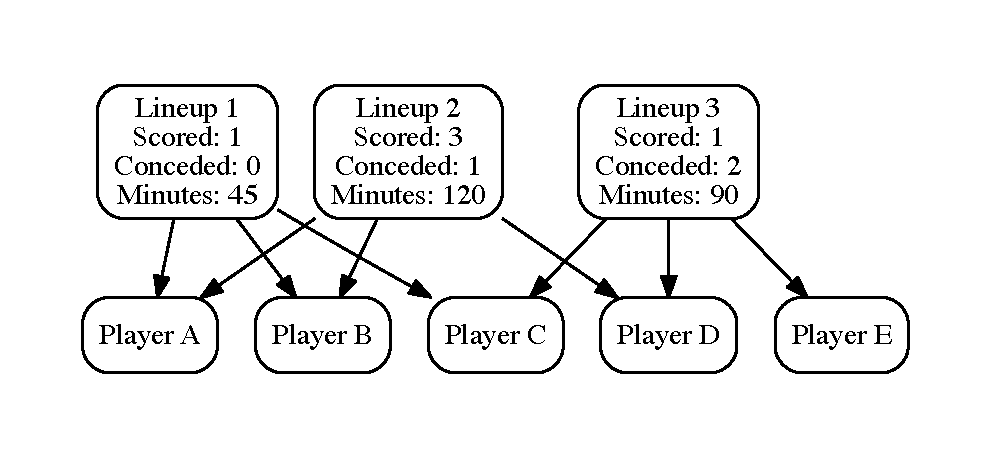
\includegraphics[width=0.9\textwidth]{graph.pdf}
    \caption{Sample graph of lineups and players. Note that this setup uses lineups of 3 players, while traditionally soccer lineups include 7-11 players.}
  \end{figure}
  
  We can think of $v(N)$ as the productivity of all Arsenal lineups. The challenge, however, is accurately dividing that productivity between Arsenal's players.
  \br
  Let us now consider a single player, Per Mertesacker, a tall, German defender for Arsenal. We can think of Mertesacker's individual payoff, $v({i})$ as the sum of the productivities of all lineups Mertesacker has participated in.
  \begin{center}
    $v({i}) = \sum\limits_{L \in {i}_{lineups}} p(L)$
  \end{center}
  More generally, the value of any coalition $S \subset N$ can be computed as follows.
  \begin{center}
    $v(S) = \sum\limits_{L \in S_{lineups}} p(L)$
  \end{center}
  It is worth noting that $S_{lineups}$ contains all unique lineups for players in $S$. If two players, both in $S$, are part of the same lineup, then $S_{lineups}$ will contain only one instance of that lineup. This fact brings up an interesting divergence from traditional cooperative games. In most cases, payoff functions are superadditive, fulfilling the following inequality.
  \begin{center}
    $v(S \cup T) \geq v(S) + v(T)$ where $S,T \subseteq N$ 
  \end{center}
  However, the soccer game as defined above is not superadditive, due to the uniqueness principle on the $S_{lineups}$ set. To illustrate this point, consider two Arsenal players, Chuba Akpom and Ryo Miyaichi. Over the 2013-2014 season, Akpom and Miyaichi have played with only one and two distinct lineups, respectively. Therefore Akpom's payoff equals the productivity of his one lineup and Miyaichi's is the sum of the productivities of his two lineups. If their lineups do not overlap, then the payoffs are superadditive---the payoff of the coalition of both Akpom and Miyaichi is equivalent to the sum of their individual payoffs. But if Miyaichi and Akpom were on the field at the same time, then their lineups overlap and their payoffs cannot be superadditive. When adding the individual payoffs, the productivity of the overlapping lineup is counted twice, while it is only counted once when considering their coalition.
  \br
  When thinking of more standard cooperative games, being non-superadditive may pose a conceptual challenge, as players would elect to compete by themselves rather than join coalitions. Since the purpose of framing soccer data as a game of this form is for a different purpose---rating the players' respective contributions---using a non-superadditive payoff function does not cause us problems, and the four axioms for determining Shapley values are still fulfilled. 
  
  \subsubsection*{Computing the Shapley Value}
  For a given team, the method for determining a player's Shapley value is theoretically identical to the above example---sum the marginal contribution of each player for each ordering of the players' payoffs. This technique is a massive computational challenge, however. Even for a single team, such as Arsenal who has had a mere 27 players appear for their squad during this season, we would have to make $27!$ ($1.0888869 * 10^{28}$) computations to determine the Shapley value of a single Arsenal player!
  \br
  There are a few ways to improve this process. One standard method is to compute symmetric players simultaneously. However, in the case of soccer players, few (if any) of them are truly symmetric.
  \br
  Another approach is to estimate the relative Shapley values of a subset of players by considering only their contributions. $N$ would become the most used 11 players, for instance, and we would consider the relative contributions of players for each ordering of these 11. It is still a computationally intensive process, requiring 39,916,800 computations for each player, but this is a far more reasonable number than what is required for the full team. The significant drawback of this approach is that it overestimates some players' productivity, specifically ones who often play with players not considered in the given subset of players. As an example, consider Wojciech Szczesny, Arsenal's Polish goalkeeper, has played along side more distinct lineups than any other Arsenal player. When computing the reduced Shapley values, Szczesny's productivity will be overestimated, because he will claim responsibility for many lineups other players will not have participated in. If Olivier Giroud and Lukas Podolski, two Arsenal forwards, often swap positions, being substituted for each other, but we only consider Olivier Giroud in our reduced computation, then Szczesny and other players who play with Podolski will absorb his contribution into their own. Giroud, however, will not be able to, since he rarely plays with Podolski.
  \br
  A more interesting technique is to calculate scores for players of the same position, because as frequent substitutes their relative value is more meaningful than comparing a defender to a forward. As examples, I computed the reduced Shapley values for Arsenal's most frequently utilized forwards, midfielders, and defenders independently, using the methodology described above. See Table 1 and Table 2 for reference.
  \br
  One way of contextualizing the relative Shapley values is by comparing them to players' weekly wages. Olivier Giroud, Mikel Arteta, Per Mertesacker, and Bacary Sagna have particularly good ratios of value to wages, while Lukas Podolski and Mesut Ozil seem to be underperforming. The Ozil case is an intriguing one, as he has been heralded as being an enormous benefit to Arsenal this season. His Shapley value is far lower than it should be with the amount the club is paying him, though. One possible explanation of his relatively low Shapley value is that he is often taken off late in games. If goals are often scored late, then he might be missing out on the effects of his hard work, wearing down the opposing defenses until his fresh-legged substitute can take advantage of them. In general, the computed values are not in contrast with wages and seem to provide another dimension in analyzing the effectiveness of individual players.  
  
  \section*{Conclusion}
  Like many sports, soccer does not lend itself well to quantitative analysis. It is very difficult to structure the little information we have about games into something resembling a useful model. Basic indicators like goals, shots, assists, and saves are easily understood and compared, but they do not adequately represent the differing contributions of players on the field. The Shapley value was developed to deal with similarly convoluted, coalitional games. I have shown how to construct a coalitional game of the data available and determined the computational intensity required to simulate values for all players on even a single team. By comparing often substituted players of the same position, we can estimate the relative values, and the results are somewhat consistent with players' weekly wage. A few exceptions seem to exist, but in general the model provides soccer with a fresh, unique method of analyzing player contributions that is rooted in collaboration, not individual play. 
  
  \newpage
  
  {\renewcommand{\arraystretch}{1.5}
  \begin{table}
    \begin{tabular*}{\textwidth}{@{\extracolsep{\fill} } l l l l l l}
      Player & Pos. & Minutes & Lineups & Value\\
      \hline
      Olivier Giroud & F & 2904.0 & 89 & 1.452397 \\
      Lukas Podolski & F & 987.0 & 33 & 0.629432 \\
      Nicklas Bendtner & F & 163.0 & 11 & 0.053889 \\
      \hline
      Kieran Gibbs & D & 2041.0 & 70 & 0.478098 \\
      Carl Jenkinson & D & 716.0 & 32 & -0.007402 \\
      Laurent Koscielny & D & 2581.0 & 91 & 0.665840 \\
      Per Mertesacker & D & 3060.0 & 106 & 0.792059 \\
      Bacary Sagna & D & 2880.0 & 102 & 0.778335 \\
      Thomas Vermaelen & D & 777.0 & 32 & 0.428788 \\
      \hline
      Mikel Arteta & M & 2281.0 & 80 & 0.929605 \\
      Santi Cazorla & M & 2519.0 & 79 & 0.544304 \\
      Alex Oxlade-Chamberlain & M & 527.0 & 25 & -0.002460 \\
      Aaron Ramsey & M & 1699.0 & 59 & 0.421665 \\
      Tomas Rosicky & M & 1478.0 & 44 & 0.305769 \\
      Theo Walcott & M & 859.0 & 35 & 0.603445 \\
      Jack Wilshere & M & 1691.0 & 60 & 0.220789 \\
      Mesut Ozil & M & 1960.0 & 54 & 0.112600 \\
    \end{tabular*}
    \caption{Arsenal FC Shapley Values By Position}
  \end{table}
  }
  
  \newpage
  
  {\renewcommand{\arraystretch}{1.5}
  \begin{table}
    \begin{tabular*}{\textwidth}{@{\extracolsep{\fill} } l l l l}
      Player & Pos. & Wage & Value \\
      \hline
      Olivier Giroud & F & \pounds60,000 & 1.452397 \\
      Lukas Podolski & F & \pounds107,000 & 0.629432 \\
      Nicklas Bendtner & F & - & 0.053889 \\
      \hline
      Kieran Gibbs & D & \pounds50,000 & 0.478098 \\
      Carl Jenkinson & D & \pounds20,000 & -0.007402 \\
      Laurent Koscielny & D & \pounds50,000 & 0.665840 \\
      Per Mertesacker & D & \pounds60,000 & 0.792059 \\
      Bacary Sagna & D & \pounds60,000 & 0.778335 \\
      Thomas Vermaelen & D & \pounds70,000 & 0.428788 \\
      \hline
      Mikel Arteta & M & \pounds70,000 & 0.929605 \\
      Santi Cazorla & M & \pounds70,000 & 0.544304 \\
      Alex Oxlade-Chamberlain & M & \pounds40,000 & -0.002460 \\
      Aaron Ramsey & M & \pounds50,000 & 0.421665 \\
      Tomas Rosicky & M & \pounds80,000 & 0.305769 \\
      Theo Walcott & M & \pounds90,000 & 0.603445 \\
      Jack Wilshere & M & \pounds60,000 & 0.220789 \\
      Mesut Ozil & M & \pounds160,000 & 0.112600 \\
    \end{tabular*}
    \caption{Arsenal FC Shapley Values and Weekly Wages}
  \end{table}
  }
  
\end{document}
